\cleardoublepage

\chapter{}
\label{chap:c}

\begin{description}[leftmargin=!,labelwidth=\widthof{\bfseries Volume and number}]
    \item[Title] Area-Averaged Transmitted and Absorbed Power Density on a Realistic Ear Model
    \item[Authors] Ante Kapetanović, Giulia Sacco, Dragan Poljak, Maxim Zhadobov
    \item[Journal] IEEE Journal of Electromagnetics, RF, and Microwaves in Medicine and Biology
    \item[Year] 2023
    \item[Volume and number] 7, 1
    \item[Pages] 39--45
    \item[Categorization] Research paper
    \item[Language] English
    \item[Keywords] Absorbed power density, electromagnetic dosimetry, millimeter waves, realistic ear model
    \item[Abstract] At millimeter waves (MMW), the current state of research in computational dosimetry is mainly relying on flat-surface tissue-equivalent models to simplify the exposure assessment by disregarding geometrical irregularities characteristic of conformal surfaces on realistic models.
    However, this can lead to errors in estimation of dosimetric quantities on non-planar body parts with local curvature radii comparable to the wavelength of the incident field.
    In this study, we address this problem by developing an averaging technique for the assessment of the absorbed power density ($S_\text{ab}$) on the anatomically-accurate electromagnetic (EM) model of the human ear.
    The dosimetric analysis is performed for the plane-wave exposure at 26 and 60 GHz, and the accuracy of the proposed method is verified by using two commercial EM software. Furthermore, we compare the two definitions of $S_\text{ab}$ provided in the international guidelines and standards for limiting exposure to EM fields above 6 GHz.
    Results show marginal relative differences between the obtained values from the two different definitions (within about 6\%) in all considered scenarios.
    On the other hand, in comparison to flat models, the spatial maximum $S_\text{ab}$ on the ear is up to about 20\% larger regardless of definition.
    These findings demonstrate a promising potential of the proposed method for the assessment of $S_\text{ab}$ on surfaces of anatomical models at frequencies upcoming for the 5th generation (5G) wireless networks and beyond.
    \item[Databases] Scopus, Google Scholar, Web of Science Core Collection -- Emerging Sources Citation Index
    \item[Impact factor] 3
    \item[DOI] \href{https://doi.org/10.1109/JERM.2022.3225380}{\url{10.1109/JERM.2022.3225380}}
    \item[Copyright notice] \copyright 2023 IEEE. Reprinted, with permission, from Ante Kapetanović, Giulia Sacco, Dragan Poljak and Maxim Zhadobov, Area-Averaged Transmitted and Absorbed Power Density on a Realistic Ear Model, IEEE Journal of Electromagnetics, RF, and Microwaves in Medicine and Biology, 2023
\end{description}

\cleardoublepage

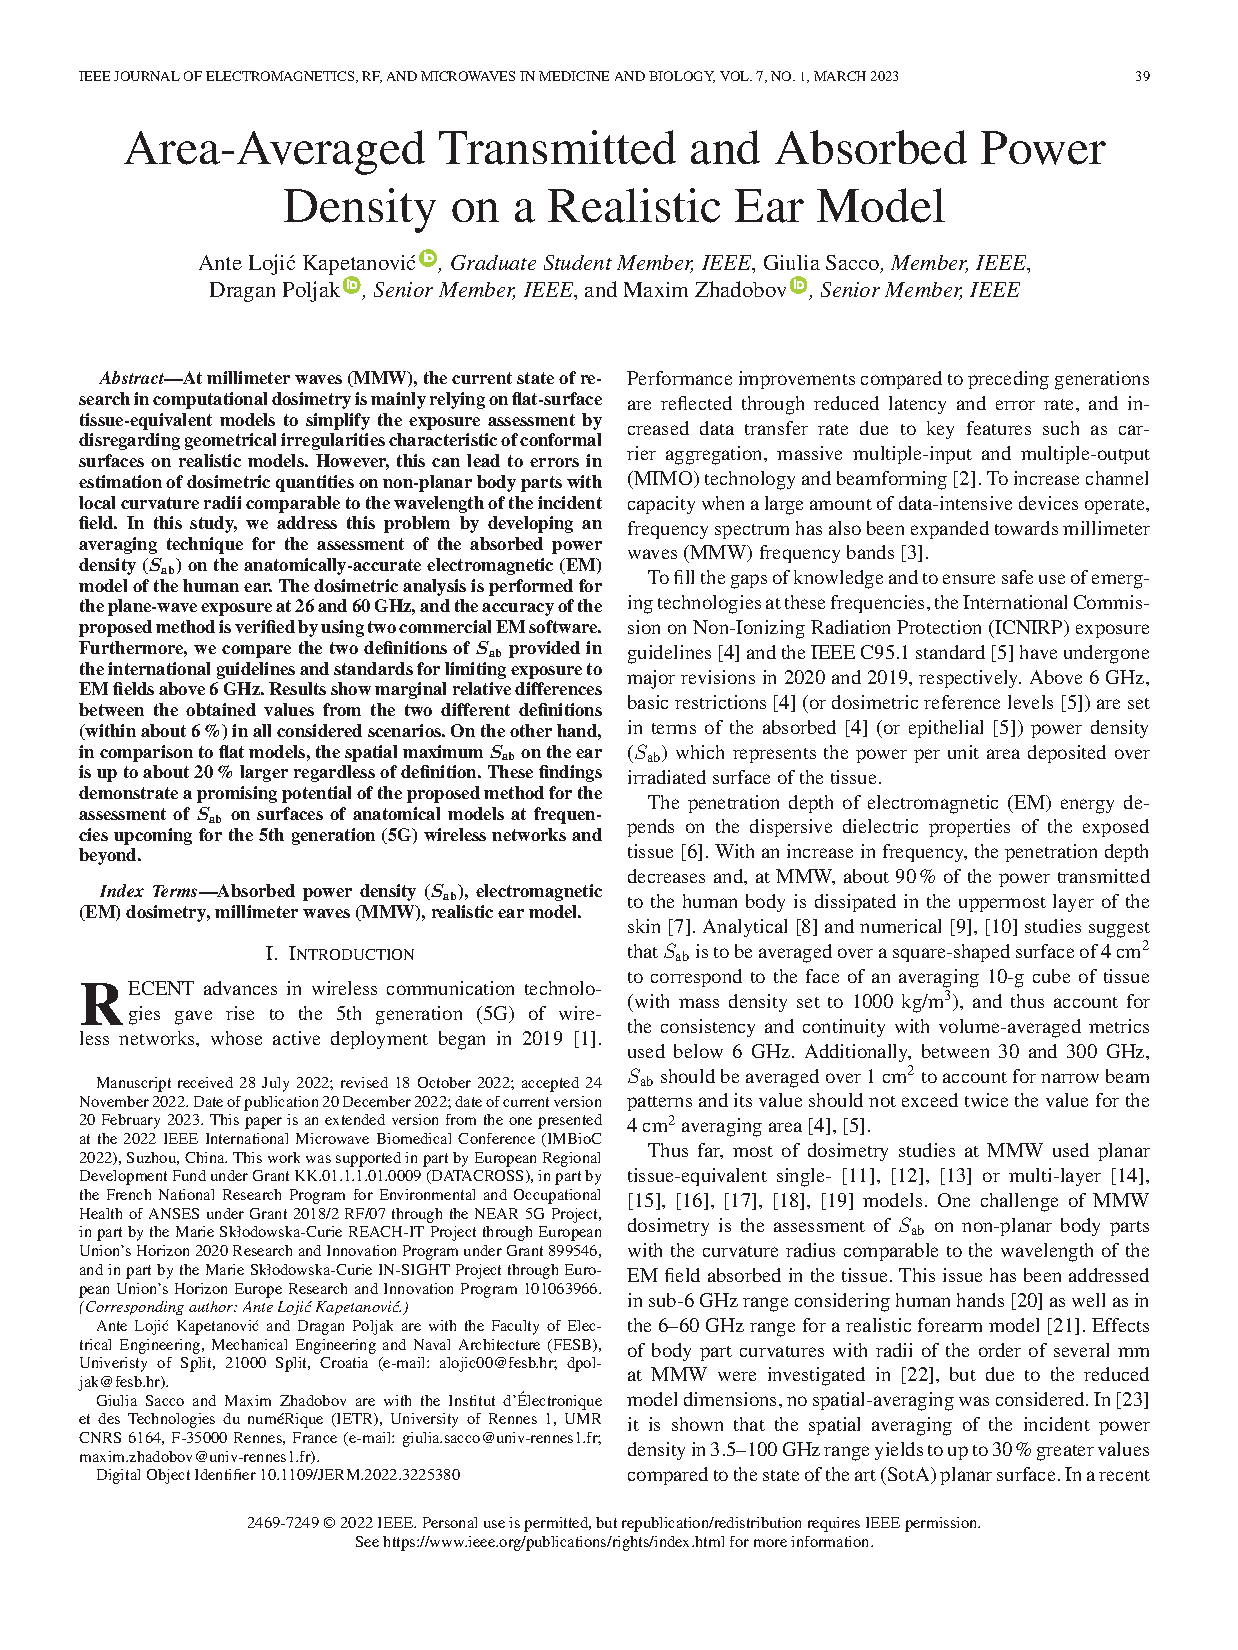
\includepdf[pages=-, pagecommand={\thispagestyle{includepdfstyle}}]{papers/Kapetanovic2023jerm.pdf}
